\tikzset{every picture/.style={line width=0.75pt}} %set default line width to 0.75pt        

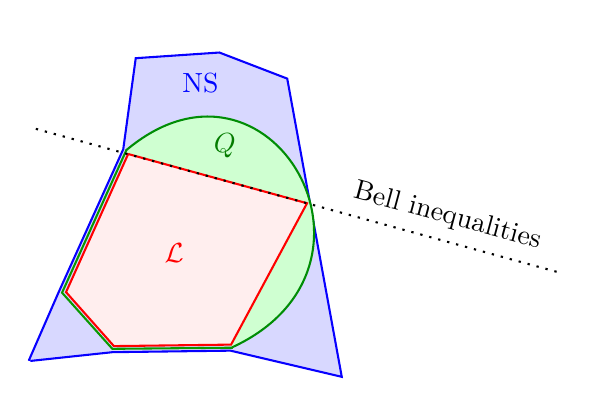
\begin{tikzpicture}[x=0.75pt,y=0.75pt,yscale=-1,xscale=1]
%uncomment if require: \path (0,300); %set diagram left start at 0, and has height of 300

%Straight Lines [id:da23136337283083197] 
\draw [color={rgb, 255:red, 7; green, 0; blue, 255 }  ,draw opacity=1 ][fill={rgb, 255:red, 216; green, 216; blue, 255 }  ,fill opacity=1 ]   (193.24,212.35) -- (232.84,208.12) -- (289.68,207.39) -- (343.3,220) -- (317.02,76.32) -- (284.32,63.75) -- (244.03,66.48) -- (238.01,110.36) -- (206.66,179.74) -- (192.47,212.25) ;


%Curve Lines [id:da7638922601289366] 
\draw [color={rgb, 255:red, 0; green, 141; blue, 5 }  ,draw opacity=1 ][fill={rgb, 255:red, 207; green, 255; blue, 209 }  ,fill opacity=1 ]   (290.45,205.8) .. controls (374.54,167.01) and (308.55,52.28) .. (239.22,111.01) ;


%Straight Lines [id:da5242020331974522] 
\draw [color={rgb, 255:red, 255; green, 0; blue, 0 }  ,draw opacity=1 ][fill={rgb, 255:red, 255; green, 238; blue, 238 }  ,fill opacity=1 ]   (240.53,112.33) -- (210.46,179.2) -- (233.52,205.2) -- (289.97,204.48) -- (326.56,136.37) -- (240.53,112.69) ;


%Straight Lines [id:da9957536132619464] 
\draw [color={rgb, 255:red, 10; green, 153; blue, 0 }  ,draw opacity=1 ]   (239.47,110.9) -- (208.53,179.47) -- (232.76,206.51) -- (290.86,205.97) ;


%Straight Lines [id:da34626836175073983] 
\draw  [dash pattern={on 0.84pt off 2.51pt}]  (195.89,100.52) -- (449.07,170.01) ;



% Text Node
\draw (262.5,160.59) node [color={rgb, 255:red, 255; green, 0; blue, 0 }  ,opacity=1 ]  {$\mathcal{L}$};
% Text Node
\draw (286.9,108.64) node [color={rgb, 255:red, 4; green, 124; blue, 0 }  ,opacity=1 ]  {$Q$};
% Text Node
\draw (275.22,78.23) node [color={rgb, 255:red, 0; green, 6; blue, 255 }  ,opacity=1 ]  {$\mathrm{NS}$};
% Text Node
\draw (394.18,142.69) node [rotate=-15.13] [align=left] {Bell inequalities};


\end{tikzpicture}